Sucede cuando las ondas se \textbf{superponen en antifase}, es decir, que estan desalineadas en crestas y valles. Esto resulta en una onda con \textbf{menor amplitud}. Tiene un efecto de \textbf{cancelación} entre las ondas.

\begin{figure}[H]
  \centering
  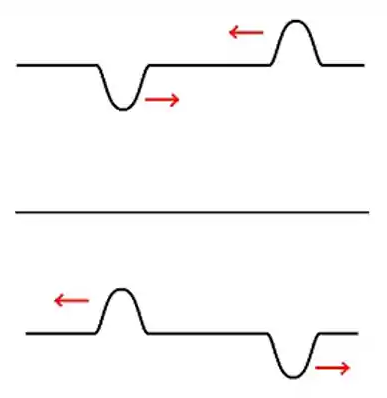
\includegraphics[scale=0.4]{imagenes/interferencia_destructiva.png}
  \caption{Interferencia destructiva\cite{respaionterf}}
\end{figure}
